\documentclass[double]{amsart}
\usepackage[margin=3cm]{geometry}                % See geometry.pdf to learn the layout options. There are lots.
\geometry{letterpaper}                   % ... or a4paper or a5paper or ... 
%\geometry{landscape}                % Activate for for rotated page geometry
\usepackage[parfill]{parskip}    % Activate to begin paragraphs with an empty line rather than an indent
\usepackage{float}
\usepackage{graphicx}
\usepackage{amssymb}
\usepackage{epstopdf}
\usepackage{setspace}
\usepackage{sidecap}
 \usepackage[table,xcdraw]{xcolor}

\DeclareGraphicsRule{.tif}{png}{.png}{`convert #1 `dirname #1`/`basename #1 .tif`.png}

\title{Lab 8: Diffraction Interference}
\author{ Caspar \textsc{Lant}} % Author name

\date{\today} % Date for the report

\begin{document}

\bigskip

\maketitle % Insert the title, author and date
\begin{center}

Intermediate Experimental Physics I\\
\vspace{1.5cm}

\begin{tabular}{l r}

Section: & 002\\
\\
Date Performed: & November 18, 2015 \\ % Date the experiment was performed
Date Due: & December 2, 2015\\
\\
Partner: & Sam P. Meier \\ % Partner names
Professor: & Prof. Andrew Kent\\ 
Instructor: & David Mykytyn % Instructor/supervisor
\end{tabular}
\end{center}
\vspace{50mm}
\pagebreak
{\setstretch{1.3}
\paragraph{\textbf{The Objective} of this week's experiment is to prove that light is a wave by means of observing constructive and destructive interference between two rays of coherent light, as well as to explore the relationship between the angle of light incident on a screen, the distance from the screen at which diffraction occurs, and the pattern projected onto the screen.}

\section{Theoretical Background/ Abstract}
\paragraph[h]{Way back in the seventeenth century, Christiann Huygens (whom we remember from our studies of pendular motion) proposed that light--that glowy thing with which we cannot do without--was a sort of wave. In the following series of experiments, we will prove him right.}
\paragraph[h!]{A pair of light waves, like all pairs of waves, can interfere with each other in a manner either constructive or destructive. Two light waves of equal wavelength, if out of phase, will interfere with one another \textit{periodically}. Consistent with its own waviness, light experiences diffraction when met with an aperture, or slit in this case, who's width is less than the wavelength of the incident light. After diffraction takes place, the once-parallel fronts of a wash of light become crescent-shaped. These crescent shaped fronts can be drawn as radial rays emanating from the diffraction slit, which interfere with each other at regular intervals. Take two waves that begin at opposite ends of the slit, and hit the screen at the same point. The difference in the distance that these two waves travel must be an integer multiple of their common wavelength for maximum constructive interference to occur. It is at these points on the screen where we see our bands of greatest intensity. Similarly, "dark points" on the screen represent positions at which the difference in distance is an odd multiple of half-wavelength; where the waves are 180$^{\circ}$ out of phase. For single-slit diffraction, these periodic areas of minima and maxima lack definition and decay quickly. The central maximum is far brighter than either of its neighboring maxima. This can be seen in the following schematic and equations: \\ }
\paragraph{}
\begin{figure}[H]
\begin{minipage}{.49\textwidth}
\centering
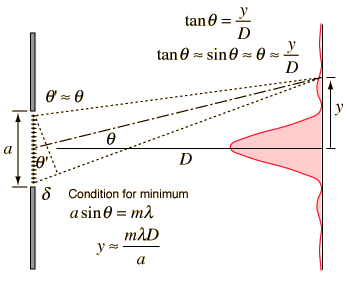
\includegraphics[width=5.5cm]{sinslit.png}
\end{minipage}
%
\begin{minipage}{.49\textwidth}
\begin{equation}
I = I_0 \left(\dfrac{\sin [\pi a  \sin \theta / \lambda]}{\pi a \sin \theta / \lambda}\right)^{2}
\end{equation}
\begin{equation} 
\sin\theta = \dfrac{m\lambda}{a}  \qquad (m = \pm1, \pm2, ...) 
\end{equation}
\end{minipage}
\end{figure}
\paragraph{Our value for wavelength can be derived through the following: $\sin\theta = \frac{m\lambda}{a} \rightarrow \lambda = \frac{a\sin\theta}{m}$, where $m =1$ for the first two maxima. $\theta$ is given by $tan^{-1}\left(\dfrac{d_{bands}}{D}\right)$, so $\lambda = a\sin\left[\tan^{-1}\dfrac{d_{bands}}{D}\right]$}
\newpage
\paragraph{Taking $\theta = 0$ in equation (1), to calculate the intensity of light at the central maxima, yields an undefined answer. With some clever math, we can take the derivative of each end of the fraction, and see that the value for intensity at $\theta = 0$ is in fact $I_0$. This is justified by L'H\^{o}pital's Rule, which states that if both sides of the fraction go to 0 or $\pm\infty$, the the limit of a fraction is equal to the limit of the derivative of the numerator, divided by the derivative of the denominator.}
\paragraph{In the case of the double-slit diffraction experiment, the bands of light projected onto the screen are much more uniform, as seen in the diagram below. The relationship between the angle of light incident on a screen, the distance from the screen at which diffraction occurs, and the intensity of the light incident on the corresponding section of screen can also be seen below.}}
\begin{figure}[H]
\begin{minipage}{.49\textwidth}
\centering
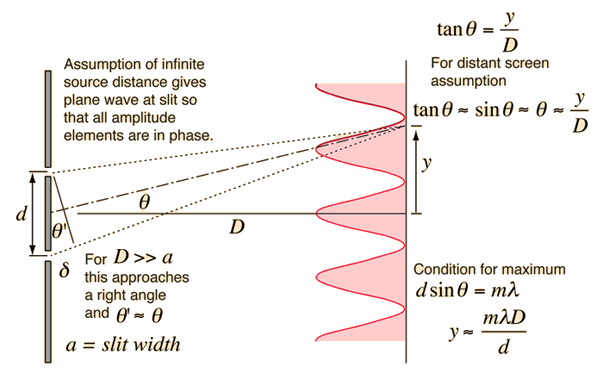
\includegraphics[width=8cm]{doubsli.png}
\end{minipage}
%
\begin{minipage}{.49\textwidth}
\begin{equation}
I = I_0 cos^2\left[\pi d \sin\left(\frac{\theta}{\lambda}\right)\right]
\end{equation}
\begin{equation}
I = I_0 cos^2\left[\pi d  \sin \theta / \lambda \right]\left(\dfrac{\sin [\pi a  \sin\theta/\lambda]}{\pi a \sin\theta / \lambda}\right)^{2}
\end{equation}
\end{minipage}
\end{figure}

 \paragraph{The derivation for wavelength in a setup with two slits goes as follows: $\sin\theta = \frac{\text{path difference}}{\text{distance between slits}}$, which for a maximum (point of constructive interference) is equal to the wavelength divided by the distance between slits, or $\lambda/d$. We know from trigonometry that $\tan\theta = \frac{d_\text{bands}}{D_\text{screen}}$, so for small values of $\theta$, $\lambda = \frac{a\cdot d_{\text{bands}}}{D}$. You'll notice that this value for wavelength does not depend on the width of the slits. }
\section{Experimental Procedure}
\begin{enumerate}
\item Attach the laser to the supplied optical bench, as in the pervious lab experiment. Turn it on. 
\item Mount a screen on the opposing end of the optical bench, making sure that it stationary and plum to the laser beam. 
\item Carefully measure the distance from the laser's aperture to the screen you have just erected. 
\item Place the slide populated with single slits on the optical bench between the laser and screen, such that the beam shines through the narrowest slit.
\item You should see a diffraction pattern projected onto the screen. Measure the distance between the middle of the central maximum (brightest point) and the first dark band. This distance is equivalent to the distance between any neighboring maxima. 
\item Reposition the slide such that the laser shines through the second slit. Measure and record the distance between maxima
\item Repeat step 6 for the third and fourth slits. 
\item Once finished, mount the slide with four pairs of slits in the path of the laser. 
\item Record the values for distance between central maxima for each pair of slits, as well as the distance between "sub maxima" between each pair of bands, if you can. 
\end{enumerate}

\section{Data Tables and Analysis}
\begin{table}[H]
\centering
\caption{My caption}
\label{my-label}
\begin{tabular}{
>{\columncolor[HTML]{FFFFFF}}c |
>{\columncolor[HTML]{FFFFFF}}c |
>{\columncolor[HTML]{FFFFFF}}c |
>{\columncolor[HTML]{EFEFEF}}c |
>{\columncolor[HTML]{EFEFEF}}c }
{\color[HTML]{333333} Width of Slits (mm)} & {\color[HTML]{333333} Distance Between Bands (mm)} & Error  in Distance(mm) & $\lambda$ (nm) & $\lambda_2$ (nm) \\ \hline
0.020                                      & 17.50                                              & $\pm$0.50              & 667.6          & 667.9            \\
0.040                                      & 8.20                                               & $\pm$0.50              & 625.9          & 626.0            \\
0.080                                      & 4.10                                               & $\pm$0.50              & 625.9          & 626.0            \\
0.160                                      & 1.90                                               & $\pm$0.50              & 580.1          & 580.2           
\end{tabular}
\\Distance Between Slits and Screen: 542mm $\pm$5mm
\end{table}
{\setstretch{1.3}
\paragraph{Computing the values for wavelength using the formula derived in section 1 leaves us with the following table. Also included are values made using the paraxial assumption: $\sin\theta\approx\tan\theta\approx\theta$. The range of values for red light, according to the French Institute of Wavelength Specification (Institut fran\c{c}ais de longueur d'onde Sp\'{e}cification) is between 620 and 750 nm, which wrap nicely around all but one of our values for wavelength.}
\paragraph{}
\begin{table}[H]
\centering
\caption{Double Slit}
\label{my-label}
\begin{tabular}{c|c|c|c}
Distance Between Slits (mm) & Width of Slits (mm) & Distance Between Bands (mm) & Error (mm) \\ \hline
0.250            & 0.04             & 9.20             & $\pm$0.50       \\
0.500            & 0.04             & 8.50             & $\pm$0.50       \\
0.250            & 0.04             & 4.00             & $\pm$0.50       \\
0.500            & 0.04             & 3.90             & $\pm$0.50      
\end{tabular}
\\Distance Between Slits and Screen: 515mm $\pm$5mm
\end{table}

\section{Error Analysis}
\paragraph{We incurred substantial error in the calculation of the laser's wavelength from the double slit data.Using the paraxial approximation, we can compute the error using the following formula, which gives us the table below. As you can see, most of our values for wavelength fall within the prescribed range of red light. The standard deviation in our first set of values, after corrections made for error, was 18.5 nanometers, or 2.87\% of the average value for wavelength. Our sources of error are hard to pin down, and few fall outside inaccuracy of measurement, which isn't very exciting to talk about. You'll notice that our error in wavelength tends to increase with slit width in, at least in the single slit experiment. The precision of our lab equipment, has some finite value, but we treat given quantities like slit width and distance of "errorless," because we are not given the value of manufacturing tolerance.}
\paragraph{}
\begin{figure}[H]
\begin{minipage}{.43\textwidth}
\begin{equation}
\delta\lambda = |\lambda||d_{slits}|\sqrt{\left( \dfrac{\delta d_\text{bands}}{d_\text{bands}} \right)^2+ \left(\dfrac{\delta D}{D}\right)^2}
\end{equation}
\end{minipage}
%
\begin{minipage}{.27\textwidth}
\begin{table}[H]
\centering
Single Slit
\begin{tabular}{c|c|c}
$\delta\lambda$ & $\lambda + \delta\lambda$ & $\lambda - \delta\lambda$ \\ \hline
0.4  & 668.0                     & 667.2                     \\
1.5  & 627.4                     & 624.3                     \\
6.1  & 632.1                     & 619.8                     \\
24.4 & 604.6                     & 555.7                    
\end{tabular}
\end{table}
\end{minipage}
%
\begin{minipage}{.27\textwidth}
\begin{table}[H]
\centering
Double Slit
\begin{tabular}{c|c|c}
$\delta\lambda$ & $\lambda + \delta\lambda$ & $\lambda - \delta\lambda$ \\ \hline
6.2             & 452.7                     & 440.4                     \\
24.5            & 849.7                     & 800.5                     \\
6.1             & 200.3                     & 188.1                     \\
24.3            & 403.0                     & 354.3                    
\end{tabular}
\end{table}
\end{minipage}
\end{figure}
\paragraph{You'll also notice that out propensity for error increased in the measurement of wavelength from the double-slit experiment. This could be due to our use of the paraxial approximation, but is more likely a result of measuring the distance between light maxima. Measuring this quantity was a difficult task, as the markings on our measuring device were spaced on a similar scale as the light bands were. To mitigate error in future trials, I would recommend using a more accurate measuring device, as well as devising a system which didn't rely on the experimenter's ability to draw a straight line without moving the screen.}
\section{Questions}

\begin{enumerate}
%
\item{\textit{Note that the forward direction, $\theta$ = 0, is maximum in intensity, not a zero. Why?}
\begin{quote}
We can use L'H\^{o}pital's Rule to compute the limit of the above equation when angle goes to zero:
$$\lim_{\theta\to0} \left( \dfrac{\lambda\sin\left[\frac{\pi a \sin\theta}{\lambda}\right]}{\pi a \sin\theta}\right)^2 = \lim_{\theta\to0}  \left( \dfrac{\frac{\partial}{\partial \theta}\lambda\sin\left[\frac{\pi a \sin\theta}{\lambda}\right]}{\frac{\partial}{\partial \theta} \pi a \sin\theta}\right)^2 = \ \ $$$$\lim_{\theta\to0} \left(\dfrac{\pi a \cos\theta \cos[\frac{\pi a \sin\theta}{\lambda}]}{\pi a \cos\theta}\right)^2 =\lim_{\theta\to0} \cos^2\left(\dfrac{\pi a \sin\theta}{\lambda}\right) = 1$$ 
\ \ \ \ \ \ \ \ \ \ \ \ \ \   $ \huge\therefore I = I_0\biggr\rvert_{\theta = 0}$ 
\end{quote}}
\medskip
\item {\textit{For what angles is the intensity zero?}
\begin{quote}
$$I = I_0 cos^2\left[\pi d  \sin \theta / \lambda \right]\left(\dfrac{\sin [\pi a  \sin\theta/\lambda]}{\pi a \sin\theta / \lambda}\right)^{2}$$
The intensity of is zero when $\sin [ \pi a \sin \theta / \lambda] = 0 $, or when $\theta = \sin^{-1}\left(\frac{m \lambda}{a}\right)$, as well as when $cos^2\left[\pi d  \sin \theta / \lambda \right] = 0$. $\cos x = 0$ when $x$ is an an odd multiple of $\pi /2 $, so $d \sin \theta/\lambda = 4a \sin\theta/\lambda = \frac{\lambda(2m -1)}{a}$. 
\[ \boxed{
$$\theta = \sin^{-1}\left(\dfrac{\lambda(2m-1)}{a} \right)$$
}\]
\end{quote}}
\end{enumerate}

\paragraph{}





}
\end{document}